\section{Thursday, July 4}

\todaybox{Today we'll finish our discussion of how to integrate around poles. We'll prove a generalized CIF which can handle poles of higher order. We'll also discuss how to handle curves that enclose multiple poles.}

We continue with another example of how to use the Cauchy Integral Formula:

\begin{ex}{}{} Let $\gamma$ be the circle of radius $2$ centered at $0$, travelled once counterclockwise. Find $\int_{\gamma} \frac{1}{z^2 + 1}dz$.

The function $\frac{1}{z^2 + 1} = \frac{1}{(z+i)(z-i)}$ has two simple poles inside the curve. So CIF doesn't immediately apply. Instead, we need to turn this into a situation where it does. Consider the following curves:


\begin{center}
\begin{tikzpicture}[baseline=(current bounding box.center)]

\draw [help lines,black!20!white] (-3,-3) grid (3,3);

\draw[red, thick, decoration={markings, mark=at position 0.5 with {\arrow{>}}},
		postaction = {decorate}] 
	([shift = (-85:56pt)] 0,0) arc (-85:85:56pt);
\draw[red, thick, decoration={markings, mark=at position 0.5 with {\arrow{>}}},
		postaction = {decorate}] 
	([shift = (95:56pt)] 0,0) arc (95:265:56pt);
	
	
	
	
\draw[blue, thick, decoration={markings, mark=at position 0.5 with {\arrow{<}}},
		postaction = {decorate}] 
	([shift = (105:20pt)] 0,1) arc (105:435:20pt);

\draw[blue, thick, decoration={markings, mark=at position 0.5 with {\arrow{<}}},
		postaction = {decorate}] 
	([shift = (-75:20pt)] 0,-1) arc (-75:255:20pt);

\draw[fill = black] (0,1) circle (2pt) node[above] {$i$};
\draw[fill = black] (0,-1) circle (2pt)node[above] {$-i$};


\draw[green, thick, decoration={markings, mark=at position 0.6 with {\arrow{>}}},
		postaction = {decorate}] 
	(0.165,1.97) -- (0.165,1.67);

\draw[green, thick, decoration={markings, mark=at position 0.6 with {\arrow{<}}},
		postaction = {decorate}] 
	(-0.165,1.97) -- (-0.165,1.67);

\draw[black, thick, decoration={markings, mark=at position 0.6 with {\arrow{<}}},
		postaction = {decorate}] 
	(0.165,-1.97) -- (0.165,-1.67);

\draw[black, thick, decoration={markings, mark=at position 0.6 with {\arrow{>}}},
		postaction = {decorate}] 
	(-0.165,-1.97) -- (-0.165,-1.67);

\draw (2,0) node[right]{$\gamma_1$};

\end{tikzpicture}
\qquad and \qquad
\begin{tikzpicture}[baseline=(current bounding box.center)]

\draw [help lines,black!20!white] (-3,-3) grid (3,3);

\draw[red, thick, decoration={markings, mark=at position 0.7 with {\arrow{>}}},
		postaction = {decorate}] 
	([shift = (85:56pt)] 0,0) arc (85:95:56pt);
\draw[red, thick, decoration={markings, mark=at position 0.7 with {\arrow{>}}},
		postaction = {decorate}] 
	([shift = (265:56pt)] 0,0) arc (265:275:56pt);
	
	
	
	
\draw[blue, thick, decoration={markings, mark=at position 0.7 with {\arrow{>}}},
		postaction = {decorate}] 
	([shift = (105:20pt)] 0,1) arc (105:75:20pt);

\draw[blue, thick, decoration={markings, mark=at position 0.7 with {\arrow{>}}},
		postaction = {decorate}] 
	([shift = (285:20pt)] 0,-1) arc (285:255:20pt);




\draw[green, thick, decoration={markings, mark=at position 0.7 with {\arrow{<}}},
		postaction = {decorate}] 
	(0.165,1.97) -- (0.165,1.67);

\draw[green, thick, decoration={markings, mark=at position 0.7 with {\arrow{>}}},
		postaction = {decorate}] 
	(-0.165,1.97) -- (-0.165,1.67);

\draw[black, thick, decoration={markings, mark=at position 0.7 with {\arrow{>}}},
		postaction = {decorate}] 
	(0.165,-1.97) -- (0.165,-1.67);

\draw[black, thick, decoration={markings, mark=at position 0.7 with {\arrow{<}}},
		postaction = {decorate}] 
	(-0.165,-1.97) -- (-0.165,-1.67);

\draw (0,2) node[above]{$\gamma_2$};
\draw (0,-2) node[below]{$\gamma_3$};

\end{tikzpicture}
\end{center}

Since none of these three curves enclose $\pm i$, CIT applies to give that:
$$\int_{\gamma_j} \frac{1}{z^2+1}dz = 0$$

\noin for each $j = 1,2,3$. Adding them together gives that:

$$0 = \sum_{j=1}^3 \int_{\gamma_j} \frac{1}{z^2+1}dz = \int_{C} \frac{1}{z^2+1}dz - \int_{C_1} \frac{1}{z^2+1}dz - \int_{C_2} \frac{1}{z^2+1}dz $$

\noin where $C$ is the large circle travelled once counterclockwise, $C_1$ is the smaller circle around $i$ travelled once counterclockwise, and $C_2$ is the smaller circle around $-i$ travelled once counterclockwise. This second equality comes from noticing that the green lines in $\gamma_1$ and $\gamma_2$ are travelled in opposite directions, so their integrals cancel out. The same is true for the black lines in $\gamma_1$ and $\gamma_3$.

So we are left with the red arcs which together make $C$, and the blue arcs which together make $-C_1$ and $-C_2$ (notice that the blue arcs are travelling clockwise!)

All together, this shows that $\int_{C}\frac{1}{z^2 + 1}dz = \int_{C_1}\frac{1}{z^2 + 1}dz + \int_{C_1}\frac{1}{z^2 + 1}dz$. We now calculate these two integrals using CIF.

For the integral around $C_1$, let $f(z) = \frac{1}{z+i}$. Then $f(z)$ is analytic on $\C\setminus\{-i\}$, which is a domain containing $C_1$ and its inside. So:

$$\int_{C_1} \frac{1}{z^2+1} dz = \int_{C_1}\frac{f(z)}{z-i}dz = 2\pi i f(i) = \pi$$

And similarly, $\int_{C_2}\frac{1}{z^2 + 1}dz = -\pi$. So all together, $\int_C \frac{1}{z^2+1}dz = 0$.
\end{ex}

This example suggests a general technique.

\begin{thmbo}{The Deformation Theorem}{deform}\index{Deformation Theorem} Let $D$ be a domain and $z_1,\dots,z_n \in D$. Suppose $\gamma$ is a piecewise smooth, positively oriented, simple closed curve in $D$ such that the inside of $\gamma$ is in $D$ and each $z_j$ is inside $\gamma$. Suppose that $f(z)$ is analytic on at least $D\setminus\{z_1,\dots,z_n\}$. Further, suppose $r_1,\dots,r_n > 0$ satisfy that $\{z\in\C||z-z_j| \le r_j\}\subset D$. Let $C_j$ be the circle of radius $r_j$ centered at $z_j$ travelled once clockwise. Then:
$$\int_{\gamma} f(z)dz = \sum_{j=1}^n \int_{C_j} f(z)dz$$
\end{thmbo}

\begin{proof} We proceed by induction. Suppose $n = 1$. Fix $\theta \in (0,\pi)$. Consider the rays $R_+ = \{z_1 + re^{i\theta}|r \ge r_j\}$ and $R_- = \{z_1 + re^{-i\theta}|r \ge r_j\}$. We have something like the following picture:


\begin{center}
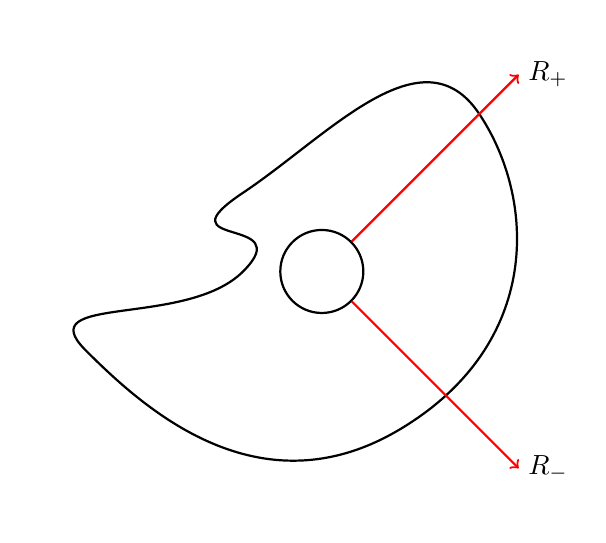
\begin{tikzpicture}

\draw[thick, ->] plot [smooth cycle, tension = 1.3] coordinates {(0,0)  (0,1) (3,2) (2,-2) (-2,-1)};
\draw[thick, <-] (1,0) circle (15pt);

\draw[thick, red,->] (1.38,0.38) -- (3.5,2.5);
\draw (3.5,2.5) node[right]{$R_+$};
\draw[thick, red,->] (1.38,-0.38) -- (3.5,-2.5);
\draw (3.5,-2.5) node[right]{$R_-$};
\end{tikzpicture}

\end{center}

Since $z_j$ is inside $\gamma$, there exists $r_+$ and $r_-$ which are the closest intersections of $R_+$ and $R_-$ with $\gamma$ to the point $z_j$. Let $L_+$ be the line segment from $z_0 + r_-e^{i\theta}$ to $z_0 + r_+e^{i\theta}$ and $L_-$ the line segment from $z_0 + r_je^{-i\theta}$ to $z_0 + r_-e^{-i\theta}$.

These intersections divide $\gamma$ into two segments: $\gamma_1$ and $\gamma_2$.  Specifcally, $\gamma_1$ starts at the intersection of $\gamma$ with $R_+$ and travels $\gamma$ in the positive orientation until it hits the intersection with $R_-$. And $\gamma_2$ starts where $\gamma$ intersects $R_-$ and travels along $\gamma$ until it hits $R_+$ 

Similarly, the circle is divided into two segments: the arc $A_1$ from the angle $-\theta$ to $\theta$, and the arc $A_2$ from the angle $\theta$ to $2\pi - \theta$.

By our construction and the assumption that $C_1$ is inside $\gamma$, $z_1$ is not inside either of $\gamma_1 - L_- - A_2 + L_+$ or $\gamma_2 - L_+ - A_1 + L_-$. (Follow the picture to see why these are the curves we want.) These are each simple closed, positively oriented curves whose insides are in $D\setminus\{z_1\}$. As such, CIT gives that:

$$\int_{\gamma_1 - L_- - A_2 + L_+} f(z)dz = \int_{\gamma_2 - L_+ - A_1 + L_-}f(z)dz = 0$$

Adding these together, we get that:

$$\int_{\gamma_1} f(z)dz - \int_{L_-}f(z)dz -\int_{A_2}f(z)dz + \int_{L_+}f(z)dz + \int_{\gamma_2} f(z)dz - \int_{L_+}f(z)dz - \int_{A_1}f(z)dz - \int_{L_1}f(z)dz = 0$$

Simplifying gives that $\int_{\gamma} f(z)dz - \int_{C_1}f(z)dz = 0$, as desired.

Proceeding with the induction, suppose the claim is true for $k$ points $z_1,\dots, z_k$ where $k\le n$.

Decompose $\gamma$ as in the case for $n = 1$. However, in this case, we will have that $\gamma_1 - L_- - A_2 + L_+$ will now have (without loss of generality) $z_2,\dots,z_k$ inside $\gamma_1 - L_- - A_2 + L_+$ for some $k\le n$. The remaining $z_{k+1},\dots,z_n$ (if there are any) will be inside $\gamma_2 - L_+ - A_1 + L_-$ necessarily. Since $\{z_2,\dots,z_k\}$ contains at most $n-1$ points, the induction hypothesis applies to give:

$$\int_{\gamma_1 - L_- - A_2 + L_+} f(z)dz = \sum_{j = 2}^k \int_{C_j} f(z)dz$$

\noin and similarly the induction hypothesis gives us that:

$$\int_{\gamma_2 - L_+ - A_1 + L_-} f(z)dz = \sum_{j = k+1}^n \int_{C_j} f(z)dz$$

Adding these two together, as in the $n=1$ case, gives:

$$\int_{\gamma} f(z)dz - \int_{C_1}f(z)dz = \sum_{j = 2}^n \int_{C_j}f(z)dz$$

Rearranging gives the desired result.
\end{proof}

As an easy consequence of this, we can state a more general version of the Cauchy Integral Formula:

\begin{corbo}{Cauchy's Integral Formula (vII)}{CIF2}\index{Cauchy's Integral Formula}
Suppose $f(z)$ is analytic on a domain $D$. Let $\gamma$ be a piecewise smooth, positively oriented, simple closed curve in $D$ whose inside is in $D$. Suppose $z_0$ is inside $\gamma$. Then:

$$\int_{\gamma} \frac{f(z)}{z-z_0}dz = 2\pi if(z_0)$$
\end{corbo}

This follows immediately from deforming $\gamma$ to a circle and using our original CIF.

\subsection{Poles of Higher Order}

Now that we know how to integrate curves surrounding a simple pole, or multiple simple poles, how do we handle integrating around higher order poles? For example, how do we find $\int_{|z|=1}\frac{e^z}{z^2}dz$? It turns out that we can generalize the CIF to handle this.

\begin{thmbo}{The Generalized Cauchy Integral Formula (or the Cauchy Differentation Formula)}{GCIF}\index{Cauchy's Integral Formula!Generalized}\index{Cauchy's Differentiation Formula}
Suppose $f(z)$ is analytic on a domain $D$. Let $\gamma$ be a piecewise smooth, positively oriented, simple closed curve in $D$ whose inside is in $D$. Suppose $z_0$ is inside $\gamma$. Suppose $n > 0$. Then:

$$\int_{\gamma} \frac{f(z)}{(z-z_0)^n}dz = \frac{2\pi i}{(n-1)!}f^{(n-1)}(z_0)$$
\end{thmbo}

The key to proving this is a result from multivariable calculus called the Leibniz Integral Rule.

\begin{lem} Suppose $f(w,z)$ is continuous in both $z$ and $w$ on some region $R$ such that if $(w_0,\gamma(t)) \in R$ for all $t$ whenever there exists $(w_0,z)\in R$. Further, suppose that $f_w(w,z)$ is continuous in both $z$ and $w$. Then:

$$\frac{d}{dw} \int_{\gamma} f(w,z)dz = \int_{\gamma} \frac{\partial}{\partial w} f(w,z)dz$$
\end{lem}

We will not be proving this. We move on to the proof of our theorem:

\begin{proof} We proceed by induction. For $n = 1$, the claim holds by the regular Cauchy Integral Formula.

Suppose the claim holds for some $n$. Let $g(z_0,z) = \frac{f(z)}{(z-z_0)^n}$. Notice that since $z_0$ is inside $\gamma$ and $z$ is on $\gamma$, that $g(z_0,z)$ is continuous in $z_0$ and $z$ (we can actually take $z$ close to $\gamma$, since $z_0$ has some positive distance between it and $\gamma$). Further:

$$\frac{\partial}{\partial z_0} g(z_0,z) = \frac{nf(z)}{(z-z_0)^{n+1}}$$

\noin is also continuous on the same region, for the same reason. As such, Leibniz's rule gives:

\begin{align*}\int_{\gamma} \frac{f(z)}{(z-z_0)^{n+1}}dz &= \int_{\gamma} \frac{1}{n} \frac{\partial}{\partial z_0} g(z_0,z) dz\\
&= \frac{1}{n}\frac{d}{dz_0}\int_{\gamma} g(z_0,z)dz\\
&= \frac{1}{n} \frac{d}{dz_0}\int_{\gamma} \frac{f(z)}{(z-z_0)^n}dz
\end{align*}

However, our induction hypothesis gives that $\int_{\gamma} \frac{f(z)}{(z-z_0)^n}dz = \frac{2\pi i}{(n-1)!}f^{(n-1)}(z_0)$. So:

\begin{align*}\int_{\gamma} \frac{f(z)}{(z-z_0)^{n+1}}dz &= \frac{1}{n}\frac{d}{dz_0}\frac{2\pi i}{(n-1)!}f^{(n-1)}(z_0)\\
&= \frac{2\pi i}{n!}f^{(n)}(z_0)
\end{align*}

\end{proof}

Note that at no point did we assume that the derivatives $f^{(n)}(z_0)$ exist. In fact, the Leibniz rule gives us that they exist, since they're equal to these integrals which do exist! As a corollary:

\begin{corbo}{Holomorphic Functions are Smooth}{}
If $f$ is holomorphic on a domain $D$, then $f$ is infinitely differentiable (otherwise known as smooth) on $D$.
\end{corbo}

Let's finish off with an example of using the generalized CIF.

\begin{ex}{}{} Let $\gamma$ be the circle of radius $2$ centered at $0$ travelled twice clockwise. Find $\int_{\gamma} \frac{\sin(z)}{(z^2+1)^2}dz$.

This function has two double poles, $z = \pm i$. Let $C$ be the circle of radius $2$ centered at $0$ travelled once clockwise. Then:

$$\int_{\gamma} \frac{\sin(z)}{(z^2+1)^2}dz = -2\int_{C}\frac{\sin(z)}{(z^2+1)^2}dz$$

By the deformation theorem:

$$\int_{C} \frac{\sin(z)}{(z^2+1)^2} dz = \int_{|z-i|=1} \frac{\sin(z)}{(z^2+1)^2}dz + \int_{|z+i|=1} \frac{\sin(z)}{(z^2+1)^2}dz$$

For the circle centered at $i$, we let $f(z) = \frac{\sin(z)}{(z+i)^2}$. Then $\frac{\sin(z)}{(z^2+1)^2} = \frac{f(z)}{(z-i)^2}$. Since $f(z)$ is analytic on $\C\setminus\{-i\}$, we can apply the generalized CIF to get:

$$\int_{|z-i|=1} \frac{\sin(z)}{(z^2+1)^2} dz = 2\pi i f'(i)$$

Now, $f'(z) = \frac{\cos(z)(z+i)^2 - 2\sin(z)(z+i)}{(z+i)^4}$, so: 
$$f'(i) = \frac{\frac{e^{-1} + e}{2}(2i)^2 - 2\frac{e^{-1} - e}{2i}(2i)}{16} = \frac{-4(e^{-1} + e) - 4(e^{-1} - e)}{32} = -\frac{1}{4e}$$

And so $\int_{|z-i|=1}\frac{\sin(z)}{(z^2+1)^2}dz = -\frac{\pi i }{2e}$.

For the circle centered at $-i$, we follow the same procedure with $g(z) = \frac{\sin(z)}{(z-i)^2}$. We find that:

$$\int_{|z+i|=1} \frac{\sin(z)}{(z^2+1)^2}dz = 2\pi i g'(-i)$$

And we calculate:

$$g'(-i) = \frac{-4\cos(-i) + 4i\sin(-i)}{16} = -4\frac{e^{i*i}}{16} = -\frac{1}{4e}$$

As such, $\int_{|z+i|=1}\frac{\sin(z)}{(z^2+1)^2}dz = -\frac{\pi i }{2e}$.

All together, $\int_{\gamma} \frac{\sin(z)}{(z^2+1)^2}dz = -2(-\frac{\pi i }{2e} -\frac{\pi i }{2e}) = \frac{2\pi i }{e} $.
\end{ex}